\documentclass[]{article}

\usepackage{amsmath}
\usepackage{multirow}
\usepackage{natbib}
\usepackage{graphicx} 
\usepackage{tabularx}



\begin{document}

\title{Latent Class Trajectories of AI-Induced Job Security: Identifying Organizational Catalysts for Professional Stability}

\author{Denario}
\date{Anthropic, Gemini \& OpenAI servers. Planet Earth.}

\maketitle
\begin{abstract}
The integration of Artificial Intelligence (AI) into the workplace prompts complex and heterogeneous employee responses regarding job security, which are often obscured by traditional analytical methods. To address this complexity, we adopt a person-centered approach, using Latent Class Analysis (LCA) on survey data from 2,603 employees in large global enterprises to identify distinct psychological trajectories based on current and expected job security. Our analysis reveals three distinct groups: a majority "Resiliently Optimistic" cohort, a "Stagnant Neutral" group, and a significant "Anxiously Declining" minority, demonstrating that perceptions of AI's impact are highly stratified. We then employ a multinomial logistic regression, using Elastic Net for feature selection, to identify the specific organizational policies, cultural attributes, and affective dispositions that predict membership in these latent classes. Membership in the "Resiliently Optimistic" class is strongly associated with structural enablers that provide employees with agency and tangible value, such as direct involvement in AI development and non-monetary incentives like peer recognition and learning certifications. Conversely, membership in the "Anxiously Declining" class is driven by deterrents such as fear of job loss and privacy concerns, which overwhelm the potential benefits of organizational support. These findings indicate that fostering psychological stability amidst technological change hinges not on abstract commitments to training, but on implementing participatory, incentive-aligned frameworks that empower employees and decouple AI-driven task evolution from perceived job displacement.
\end{abstract}








\section{Introduction}
\label{sec:intro}
The integration of Artificial Intelligence (AI) into the global economy marks a significant technological inflection point, distinguished from prior automation waves by its capacity to engage with cognitive tasks previously exclusive to human intellect. This advancement introduces a fundamental ambiguity into the workplace, where the potential for augmented productivity and innovation coexists with the specter of skill obsolescence and job displacement. For employees, this transition generates a complex psychological landscape of uncertainty, hope, and anxiety. Consequently, the central challenge for contemporary organizations is not merely to adopt new technologies, but to navigate this transition in a manner that harnesses the benefits of AI while cultivating workforce stability and psychological well-being. Understanding the diverse ways employees perceive AI's impact on their professional future is a critical first step in this process.

Prevailing analyses of AI's effect on job security often rely on variable-centered methods that measure aggregate shifts in employee sentiment. While useful for macroeconomic forecasting, such approaches treat the workforce as a monolithic entity and risk obscuring crucial underlying dynamics. An average measure of job security might remain stable, for instance, while masking a growing polarization between a cohort of employees who feel empowered by AI and another that feels increasingly threatened. This heterogeneity is not random noise but reflects distinct psychological trajectories shaped by personal dispositions, job roles, and, critically, the organizational environment. Without a granular understanding of these divergent response patterns, policies designed to support employees during this transition risk being misaligned, inefficient, or altogether ineffective, failing to address the specific anxieties and aspirations of distinct workforce segments.

This paper addresses this analytical gap by adopting a person-centered approach to model the heterogeneity in employee responses to AI. We move beyond conventional methods to ask whether distinct, unobserved subgroups of employees can be identified based on their perceived job security trajectories. To achieve this, we apply Latent Class Analysis to survey data from a large sample of employees, using the joint distribution of their current and three-year expected job security as indicators. This statistical method allows us to empirically derive and characterize distinct cohorts from the data, revealing a more nuanced typology of workforce adaptation. Our analysis uncovers three primary groups: a "Resiliently Optimistic" class experiencing high and stable security, an "Anxiously Declining" class perceiving a significant threat, and a "Stagnant Neutral" class marked by uncertainty.

Having identified these distinct trajectories, our primary objective is to determine which organizational factors predict an employee's membership in one class over another. We hypothesize that an organization's policies and culture function as active catalysts that can steer employees toward either resilience or anxiety. Using a multinomial logistic regression model, we investigate the influence of specific, actionable organizational levers, including direct employee involvement in AI development, the nature of training programs, non-monetary incentives, and prevailing cultural attributes. By isolating the policies most strongly associated with positive psychological outcomes, this study provides a data-driven framework for organizations seeking to decouple technological advancement from job insecurity. Ultimately, our work aims to shift the discourse from speculating whether AI will replace jobs to understanding how organizations can proactively construct an environment where employees and AI can coexist productively and securely.

\section{Methods}
\label{sec:methods}
\subsection{Sample and data}
The analysis is based on survey data collected from a sample of 2,603 employees working in large global enterprises. The survey captured a wide range of variables, including demographic information, perceptions of AI's impact on job security, affective responses to AI, and detailed assessments of organizational policies and culture. Key variables included Likert-scale items measuring current and expected job security, binary items on emotional attitudes, and questions regarding specific organizational enablers and deterrents related to AI adoption.

\subsection{Latent class analysis}
To identify unobserved heterogeneity in employee responses to AI, we employed a person-centered approach using Latent Class Analysis (LCA). The LCA was performed on the joint distribution of two indicator variables: current perceived impact of AI on job security and the expected impact in three years. This method allows for the empirical identification of distinct subgroups, or latent classes, of employees who share similar response patterns, representing different psychological trajectories.

The optimal number of classes was determined by fitting models with two to six classes and comparing their statistical fit indices. We primarily relied on the Bayesian Information Criterion (BIC), where a lower value indicates a better model fit, and the normalized entropy, which measures the certainty of classification. A three-class solution was selected as it provided the lowest BIC value and high class separation, indicating a robust and interpretable typology of employee trajectories.

\subsection{Analytical strategy}
Our analytical strategy proceeded in three main stages following the identification of the latent classes.

\subsubsection{Dimensionality reduction of affective dispositions}
To model employees' underlying emotional attitudes towards AI without introducing multicollinearity from the 16 binary survey items, we first conducted an Exploratory Factor Analysis (EFA). Given the binary nature of the items, the EFA was based on a tetrachoric correlation matrix. A Varimax rotation was applied to the extracted factors to improve interpretability. This process yielded two distinct and internally consistent latent factors, labeled "Positive Affect" and "Negative Affect". The internal consistency of these factors was assessed using McDonald's Omega ($\Omega$). The resulting factor scores were retained as continuous covariates for subsequent regression models.

\subsubsection{Predictor selection and regression modeling}
To identify the most salient organizational factors predicting class membership, we first used an Elastic Net logistic regression. This regularization method performs automated feature selection, making it well-suited for identifying a parsimonious set of predictors from a larger pool of correlated variables, such as the various organizational policies surveyed.

The predictors identified by the Elastic Net, along with the affective disposition factor scores and key deterrents, were then included in a comprehensive Multinomial Logistic Regression (MNLogit) model. The dependent variable for this model was the three-level latent class membership. The "Anxiously Declining" class was set as the reference category to facilitate the interpretation of model coefficients. This allowed us to directly estimate how specific organizational enablers and deterrents affect the odds of an employee belonging to the "Resiliently Optimistic" or "Stagnant Neutral" class compared to the most vulnerable group. Results are reported as Odds Ratios (OR) with corresponding 95\% confidence intervals.

\subsubsection{Policy simulation and robustness checks}
To translate the regression results into practical insights, we conducted a Monte Carlo policy simulation based on the estimated coefficients from the multinomial model. This simulation calculated the predicted probability of an average employee belonging to the "Resiliently Optimistic" class under different combinations of key organizational policies, specifically contrasting the effects of providing training with direct employee involvement in AI development.

Finally, to ensure the stability of our findings, we performed several robustness checks. We assessed multicollinearity among the predictors in our final model by calculating Variance Inflation Factors (VIF). Furthermore, we conducted a sensitivity analysis by re-estimating the multinomial logistic regression on modified versions of the sample: one excluding respondents who answered "Not sure" to the job security questions, and another where "Not sure" responses were imputed with the modal value. The stability of the key predictors' odds ratios across these model specifications was used to confirm the robustness of our conclusions.

\section{Results}
\label{sec:results}
Our analysis proceeds in several stages, beginning with the identification of distinct employee trajectories using Latent Class Analysis (LCA), followed by an examination of the organizational and psychological factors that predict membership in these classes.

\subsection{Latent class trajectories of AI-induced job security}
To identify unobserved heterogeneity in employees' perceptions of AI's impact on their job security, we conducted an LCA on the joint distribution of current and expected job security. We evaluated models with two to six latent classes, using the Bayesian Information Criterion (BIC) and normalized entropy to determine the optimal solution. As shown in Figure \ref{fig:lca_selection}, the three-class solution provided the optimal fit to the data. This model yielded the lowest BIC value (14,592.21) and a strong normalized entropy of 0.8032, indicating a parsimonious fit with excellent class separation and classification certainty.

\begin{figure}[h!]
    \centering
    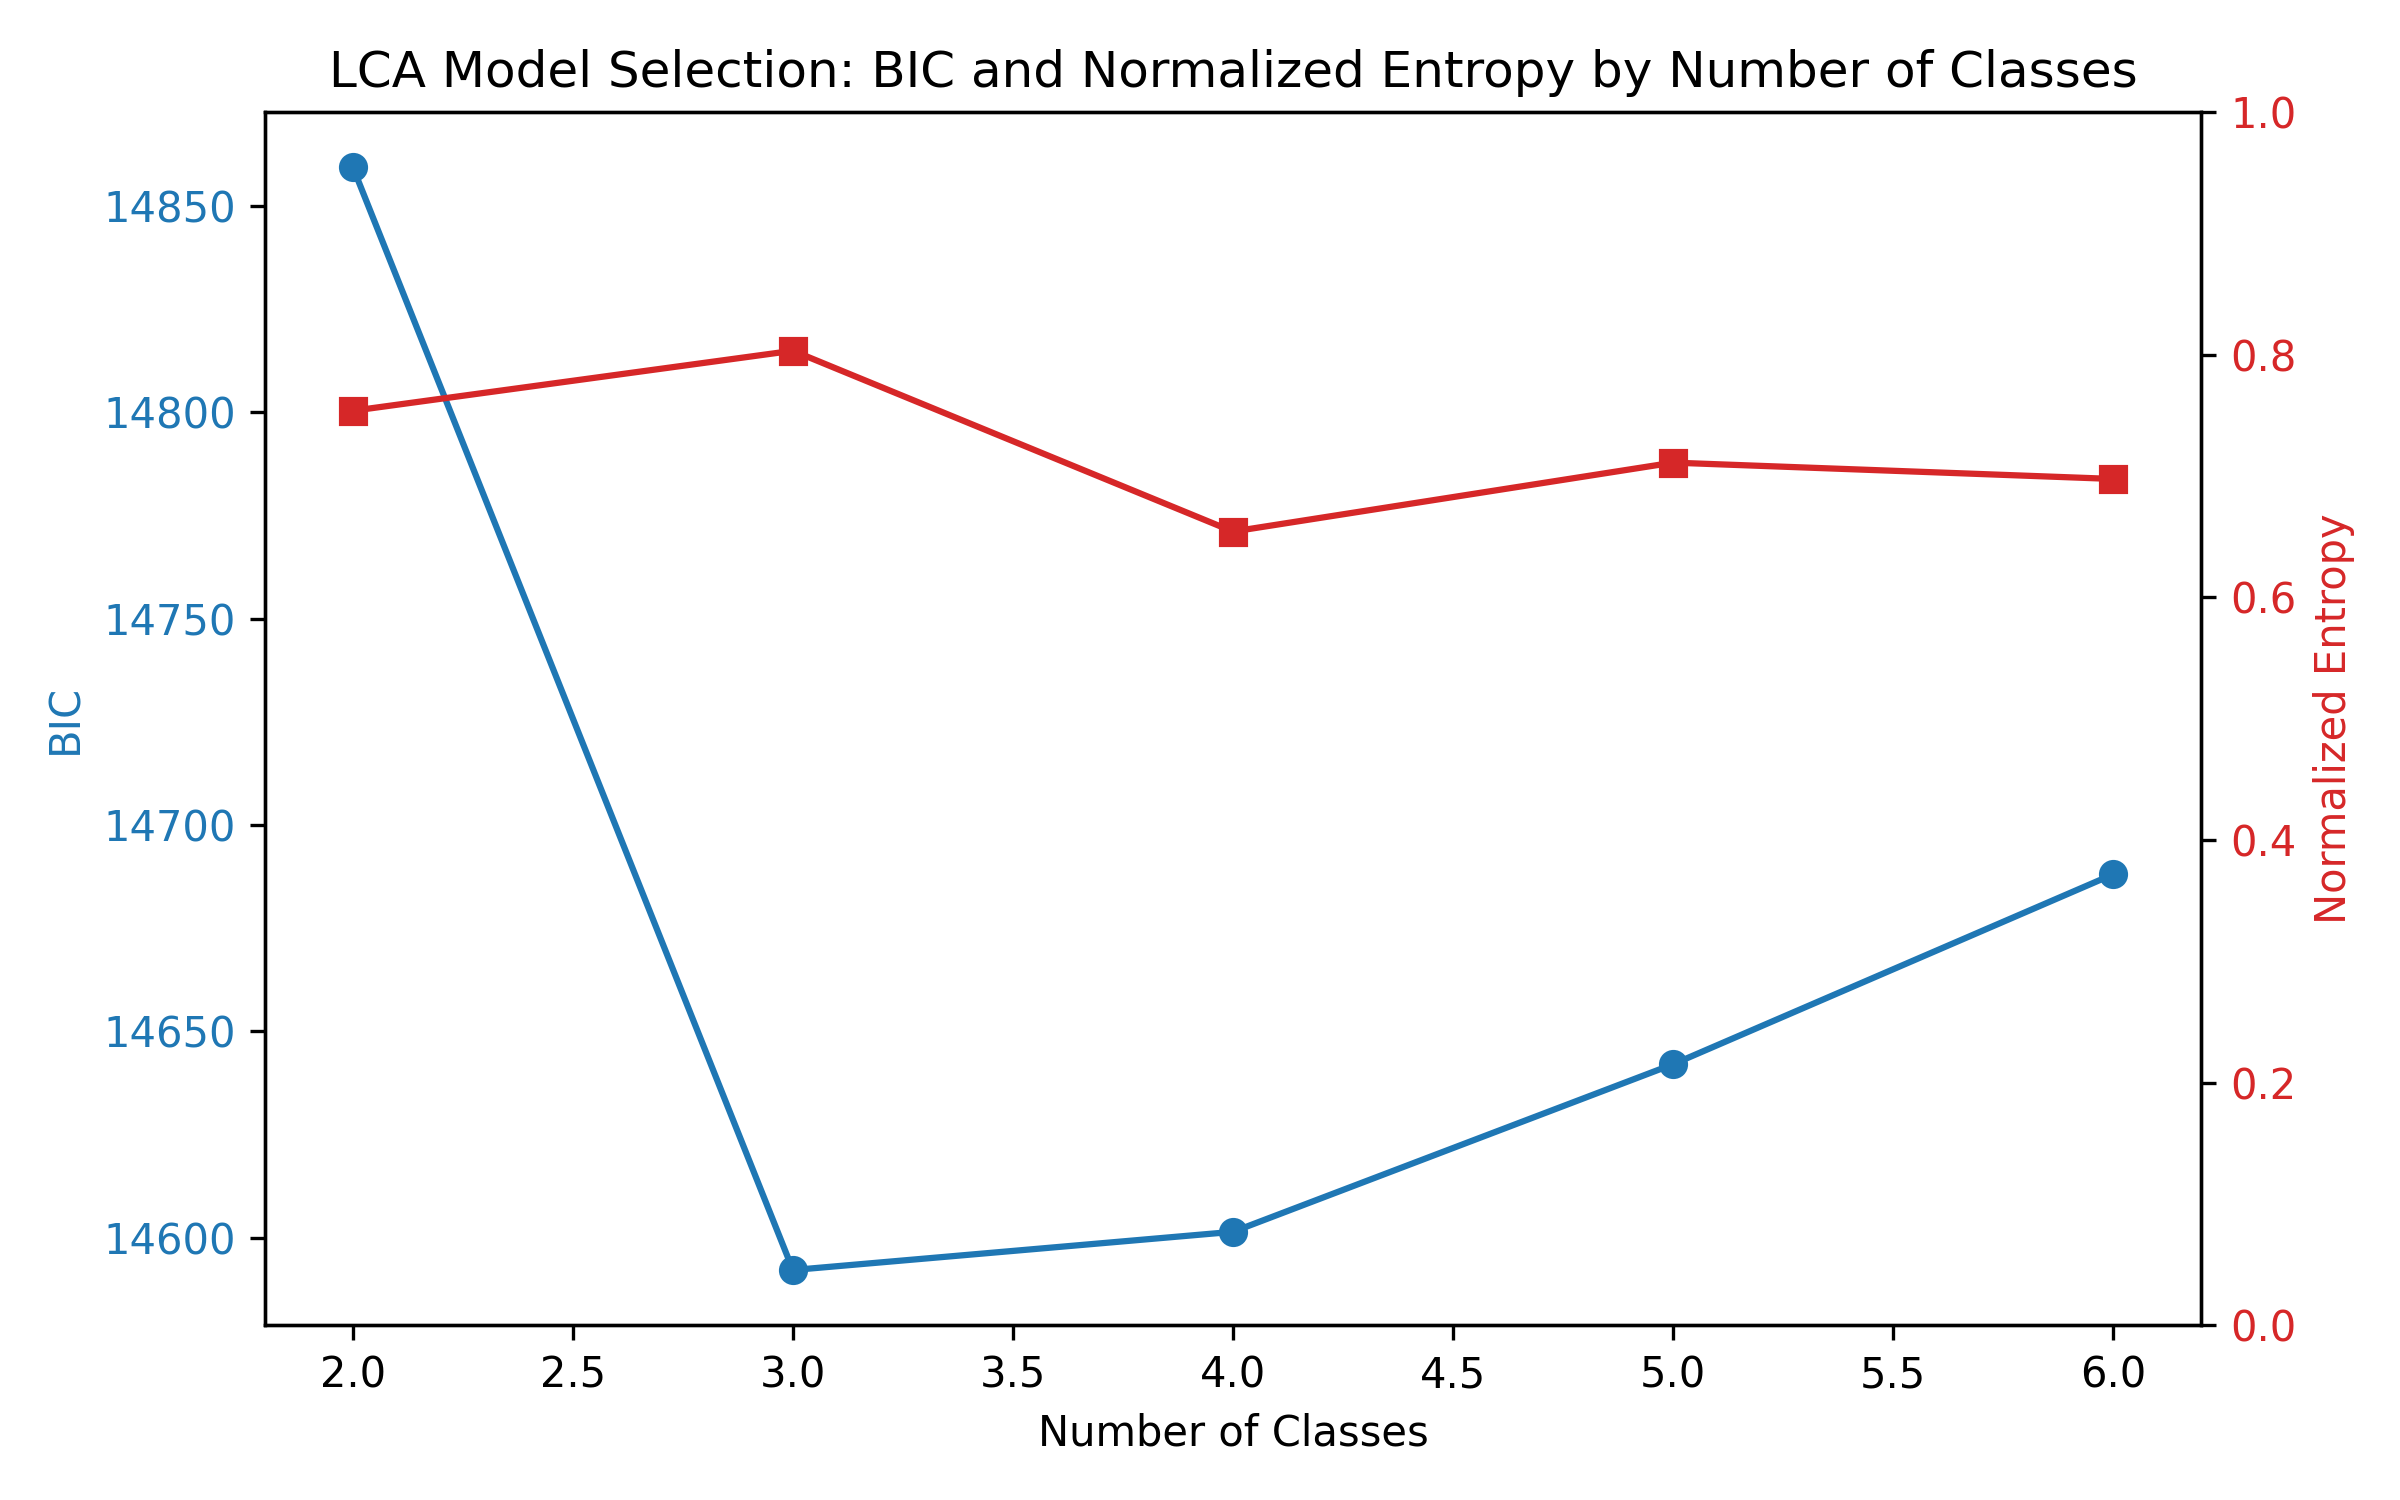
\includegraphics[width=0.6\textwidth]{../input_files/plots/step_2_lca_bic_entropy_1776114673.png}
    \caption{Model selection metrics for the Latent Class Analysis (LCA) of AI-induced job security perceptions. The plot displays the Bayesian Information Criterion (BIC; blue line) and normalized entropy (red line) for models with two to six latent classes. The three-class solution was selected as the optimal model, as it exhibits the lowest BIC value and a high normalized entropy, indicating the best balance of model fit and parsimony with clear class separation.}
    \label{fig:lca_selection}
\end{figure}

The three emergent classes represent distinct psychological trajectories:
\begin{itemize}
    \item \textbf{Class 1: "Resiliently Optimistic" (60.9\% of the sample):} This majority class is characterized by a highly positive outlook. Members of this group overwhelmingly report that AI has a positive impact on their current job security and expect this trend to continue.
    \item \textbf{Class 2: "Stagnant Neutral" (26.5\% of the sample):} This class exhibits a strong anchoring to the status quo. These employees report that AI has had no impact on their job security and largely expect this to remain the case.
    \item \textbf{Class 3: "Anxiously Declining" (12.6\% of the sample):} This minority class perceives AI as a direct threat. Members report a negative current impact on their job security and anticipate that this negative impact will persist or worsen.
\end{itemize}

The conditional response probabilities for each class, detailed in Table \ref{tab:lca_probs}, provide a granular view of these trajectories. For instance, individuals in the "Resiliently Optimistic" class have a cumulative probability of 84.2\% of reporting a positive current impact, while those in the "Anxiously Declining" class have a 92.4\% probability of reporting a negative current impact.

\begin{table*}[t]
\centering
\caption{LCA Class Sizes and Conditional Response Probabilities for the 3-Class Solution.}
\label{tab:lca_probs}
\resizebox{\textwidth}{!}{
\begin{tabular}{l|cccccc|cccccc}
\hline
\hline
& \multicolumn{6}{c|}{\textbf{Current Impact on Job Security}} & \multicolumn{6}{c}{\textbf{Expected Impact on Job Security (3 years)}} \\
\textbf{Latent Class} & Sig. Neg. & Sl. Neg. & No Impact & Sl. Pos. & Sig. Pos. & Not Sure & Sig. Neg. & Sl. Neg. & No Impact & Sl. Pos. & Sig. Pos. & Not Sure \\
\hline
\textbf{1. Resiliently Optimistic} & 0.000 & 0.030 & 0.124 & 0.419 & 0.423 & 0.004 & 0.000 & 0.046 & 0.120 & 0.377 & 0.449 & 0.008 \\
(60.90\%) & & & & & & & & & & & & \\
\textbf{2. Stagnant Neutral} & 0.000 & 0.051 & 0.861 & 0.052 & 0.000 & 0.037 & 0.000 & 0.152 & 0.628 & 0.173 & 0.000 & 0.047 \\
(26.51\%) & & & & & & & & & & & & \\
\textbf{3. Anxiously Declining} & 0.222 & 0.701 & 0.041 & 0.036 & 0.000 & 0.000 & 0.296 & 0.510 & 0.130 & 0.064 & 0.000 & 0.001 \\
(12.59\%) & & & & & & & & & & & & \\
\hline
\end{tabular}
}
\end{table*}

\subsection{Dimensionality reduction of affective dispositions}
To model employees' underlying emotional attitudes towards AI without introducing multicollinearity in subsequent models, we performed an Exploratory Factor Analysis (EFA) on 16 binary items. The analysis, using a tetrachoric correlation matrix and Varimax rotation, successfully extracted two distinct latent factors. As visualized in Figure \ref{fig:factor_loadings}, these factors clearly represent "Positive Affect" (e.g., 'optimistic', 'empowered', 'motivated') and "Negative Affect" (e.g., 'worried', 'threatened', 'anxious'). Both factors demonstrated high internal consistency, with McDonald's Omega values of 0.9004 for Positive Affect and 0.9011 for Negative Affect.

Further validation confirmed that the 'Negative Affect' factor was significantly associated with key deterrents to AI adoption, showing correlations with distrust of AI accuracy ($r = -0.246, p < 0.001$), fear of job loss ($r = -0.173, p < 0.001$), and privacy concerns ($r = -0.127, p < 0.001$). This confirms that the latent factor effectively captures underlying psychological frictions related to AI integration. The resulting factor scores were used as continuous covariates in subsequent models.

\begin{figure}[h!]
    \centering
    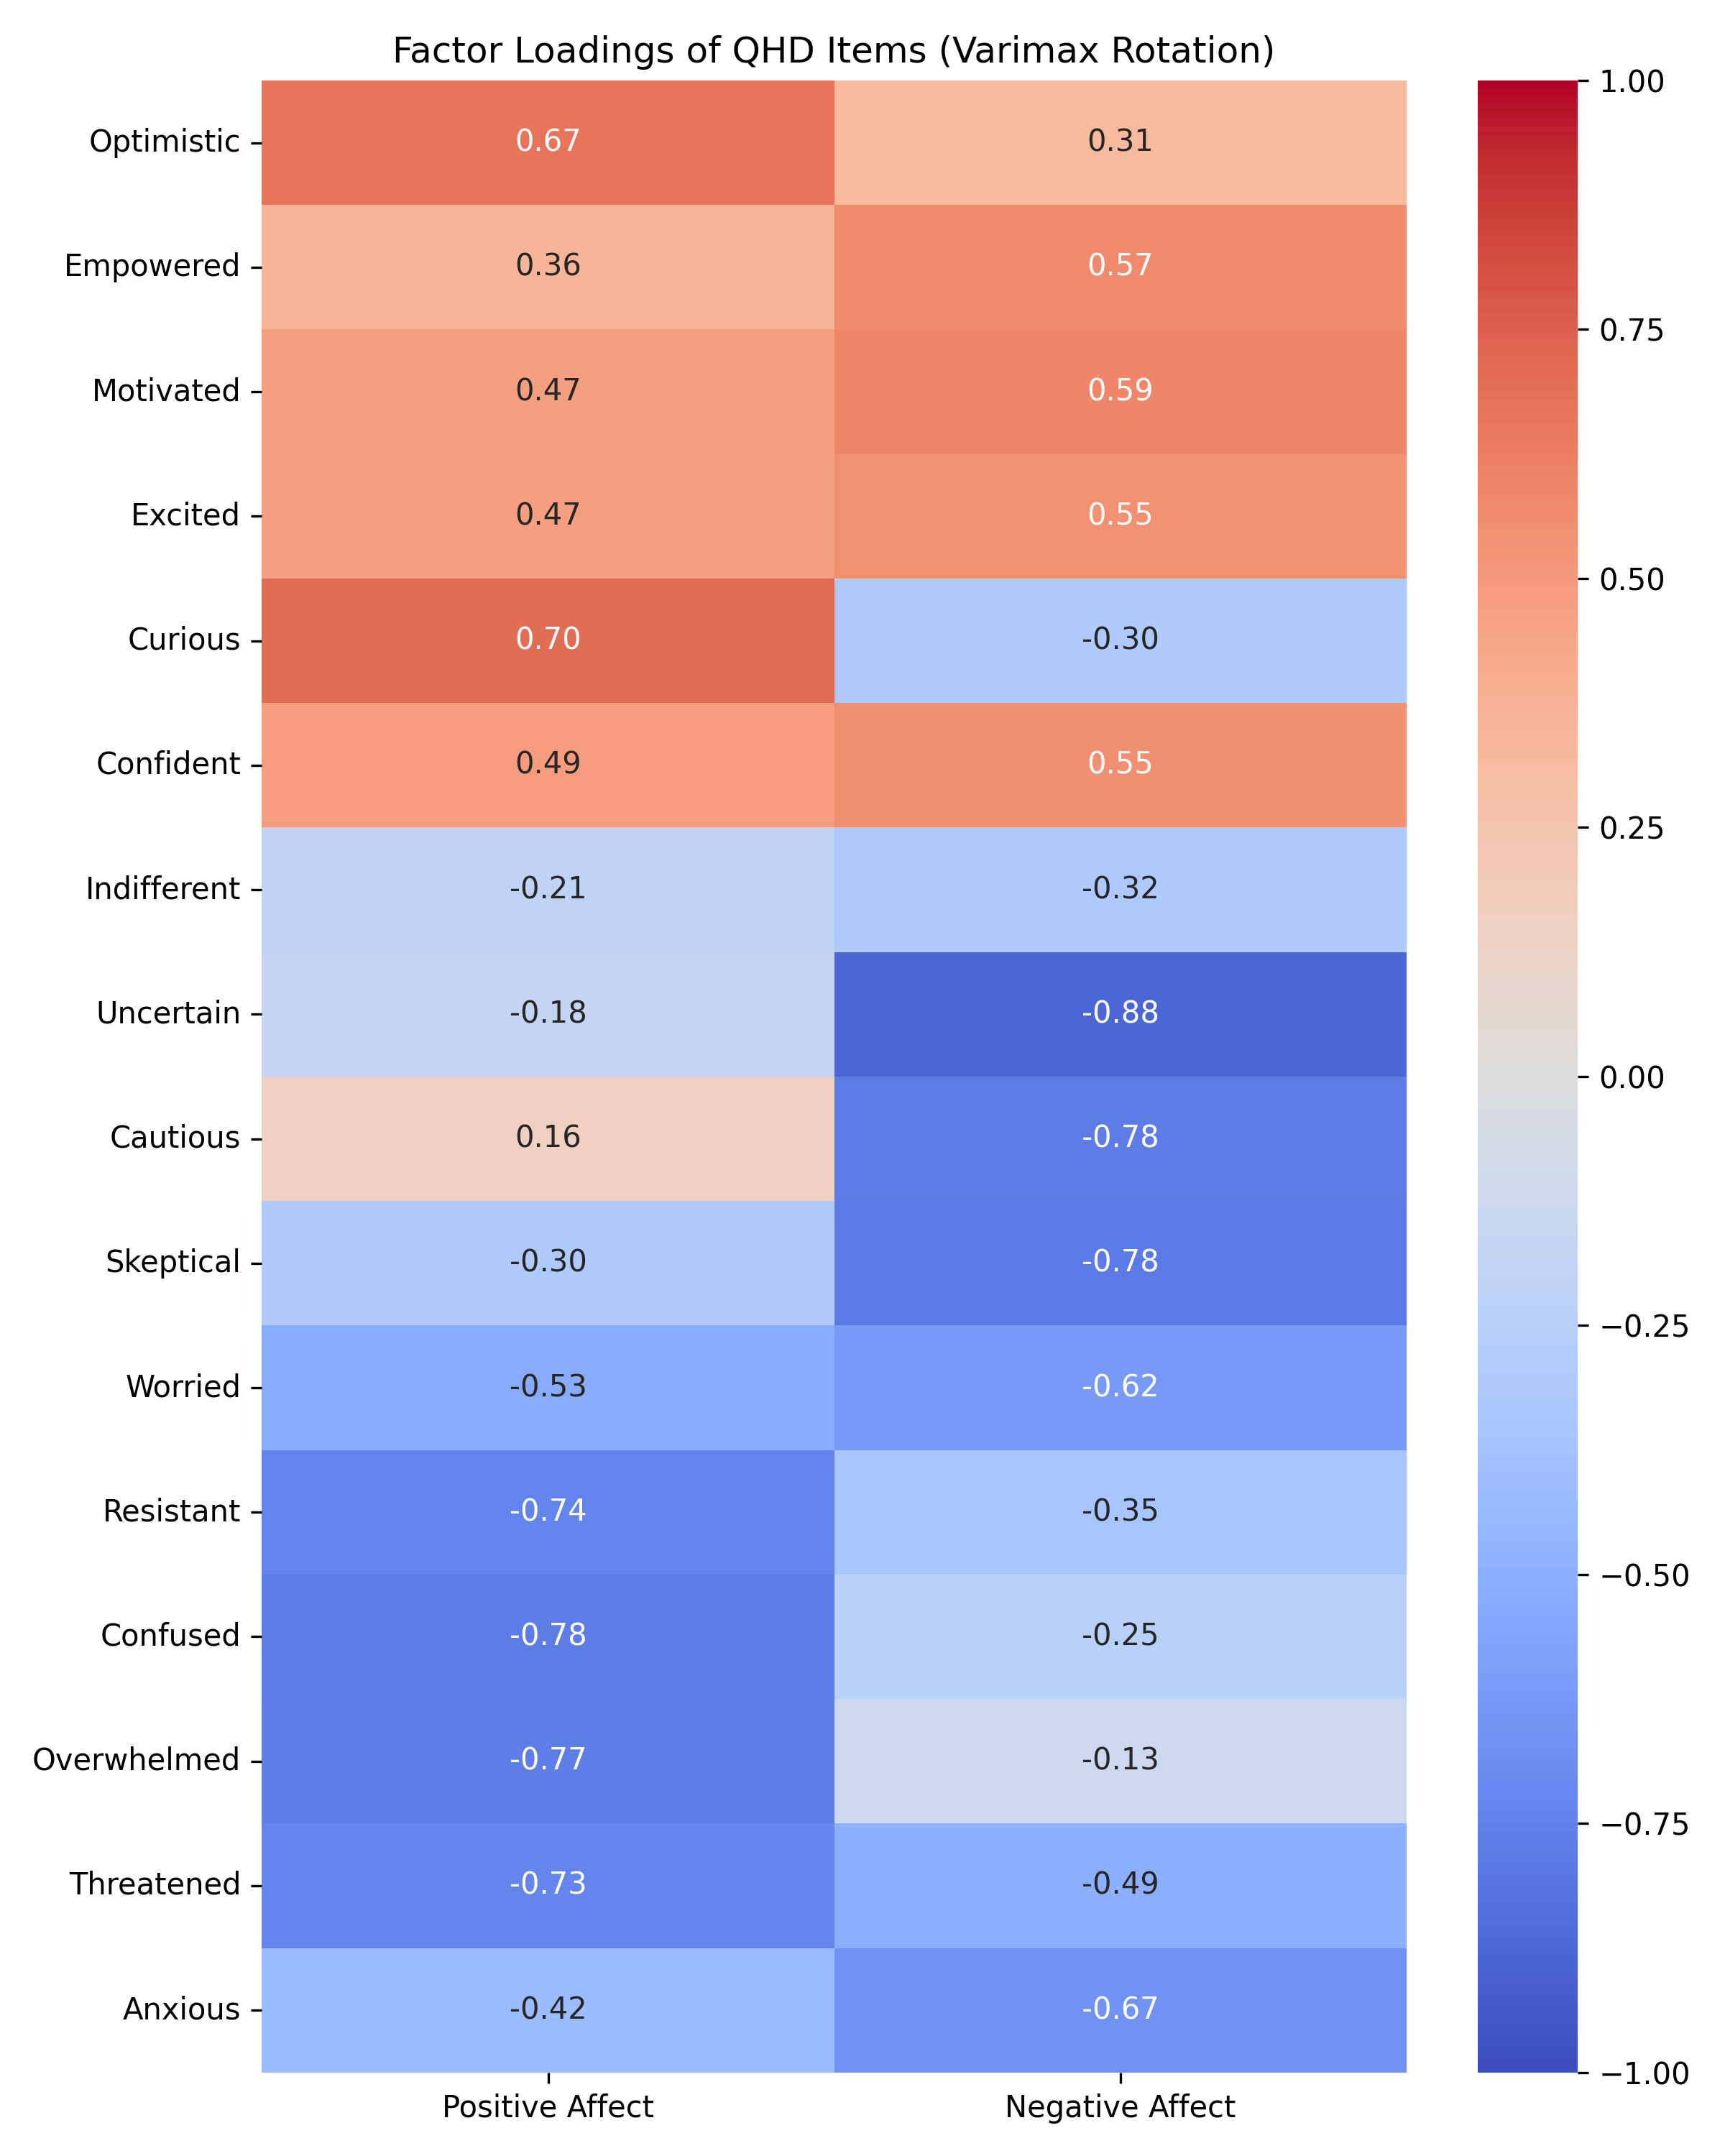
\includegraphics[width=0.6\textwidth]{../input_files/plots/step_3_qhd_factor_loadings_1776114809.png}
    \caption{Heatmap of factor loadings from an Exploratory Factor Analysis on 16 emotional attitude items after a Varimax rotation. The analysis reveals two distinct latent factors. The first factor, "Positive Affect," is strongly loaded by items such as 'Optimistic' and 'Motivated'. The second factor, "Negative Affect," is characterized by items like 'Uncertain', 'Skeptical', and 'Anxious', confirming the successful reduction of emotional attitudes into two coherent constructs.}
    \label{fig:factor_loadings}
\end{figure}

\subsection{Identifying key organizational predictors with elastic net}
We next employed an Elastic Net logistic regression to identify the most salient organizational policies and cultural attributes predicting membership in the "Resiliently Optimistic" class. This method performs automated feature selection, isolating the most impactful predictors from a larger set of correlated variables.

The results, shown in Figure \ref{fig:elastic_net}, reveal that organizational catalysts for optimism are concentrated around incentive structures and employee agency. The strongest positive predictors were non-monetary incentives, such as peer recognition ($\beta = 0.303$) and learning benefits or certifications ($\beta = 0.236$). Structural enablers that provide employees with agency, such as direct involvement in the AI development process ($\beta = 0.129$) and the freedom to choose AI tools ($\beta = 0.124$), were also highly significant. Conversely, the strongest negative predictors were deterrents rooted in risk and uncertainty, namely distrust in AI accuracy ($\beta = -0.158$) and privacy concerns ($\beta = -0.141$). Notably, the stated importance of regular training yielded a coefficient of zero, suggesting that abstract commitments to training, without tangible incentives or participatory frameworks, are insufficient to foster optimism.

\begin{figure}[h!]
    \centering
    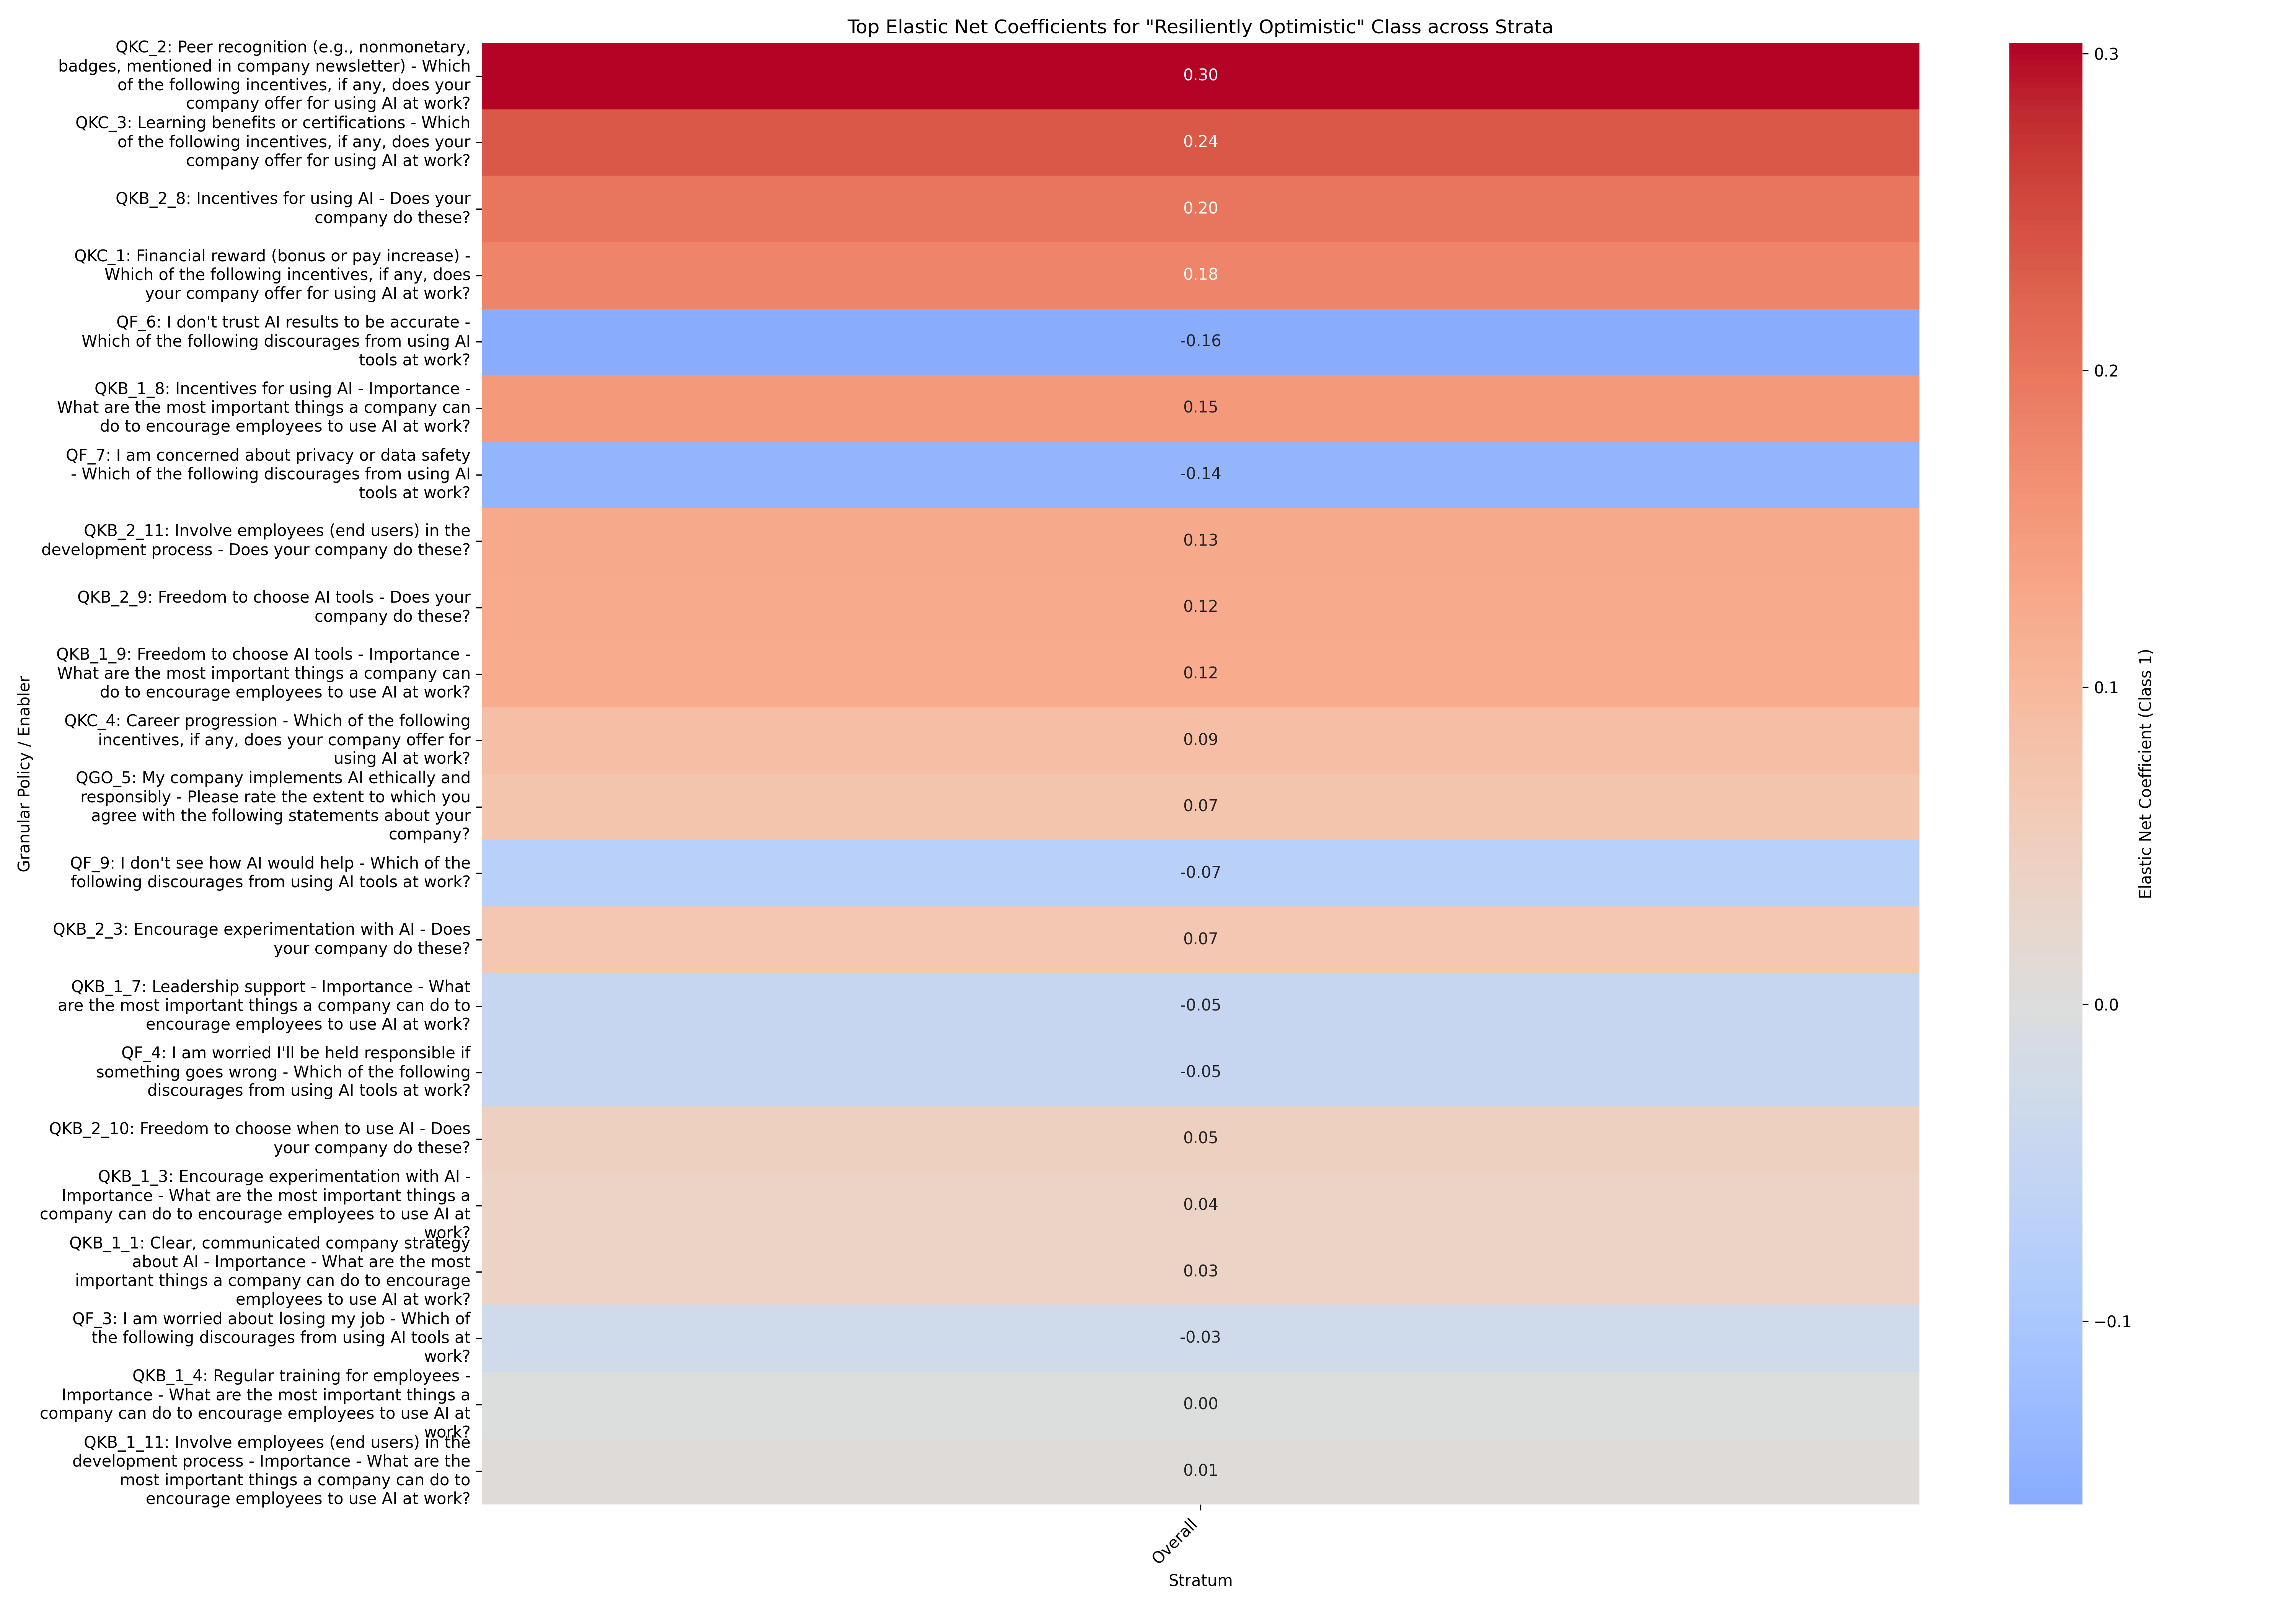
\includegraphics[width=0.6\textwidth]{../input_files/plots/step_4_elastic_net_coefficients_1776115025.png}
    \caption{Elastic Net logistic regression coefficients identifying predictors of membership in the "Resiliently Optimistic" class. Non-monetary incentives (e.g., peer recognition, learning benefits) and structural enablers (e.g., employee involvement) are the most potent positive predictors. Conversely, deterrents such as distrust in AI accuracy and privacy concerns are the strongest negative predictors.}
    \label{fig:elastic_net}
\end{figure}

\subsection{Multinomial logistic regression of class membership}
Building on the feature selection, we estimated a multinomial logistic regression model to evaluate the adjusted odds of membership in the "Resiliently Optimistic" or "Stagnant Neutral" classes relative to the "Anxiously Declining" reference class. The model included key organizational enablers, deterrents, and their interactions.

The odds ratios, visualized in Figure \ref{fig:odds_ratios}, confirm and extend the Elastic Net findings. Organizational enablers significantly increased the odds of belonging to the "Resiliently Optimistic" class. For example, providing career progression incentives increased the odds by 15.6\% (OR = 1.156), while direct employee involvement in AI development increased them by 11.1\% (OR = 1.111). The most powerful determinant was the fear of job loss; employees who cited this as a deterrent had their odds of being in the optimistic class reduced by over 82\% (OR = 0.174) compared to those who did not.

The model also revealed significant interaction effects. First, the freedom to choose AI tools was found to buffer the negative impact of privacy concerns; granting employees autonomy over tool selection significantly weakened the negative effect of privacy anxieties on their odds of being optimistic (OR for interaction = 1.281). Conversely, a second interaction showed that emphasizing the importance of regular training in a context where employees fear accountability for AI-related mistakes may exacerbate anxiety. This combination significantly reduced the odds of belonging to the optimistic class (OR for interaction = 0.712), suggesting that training initiatives must be paired with supportive accountability frameworks.

\begin{figure}[h!]
    \centering
    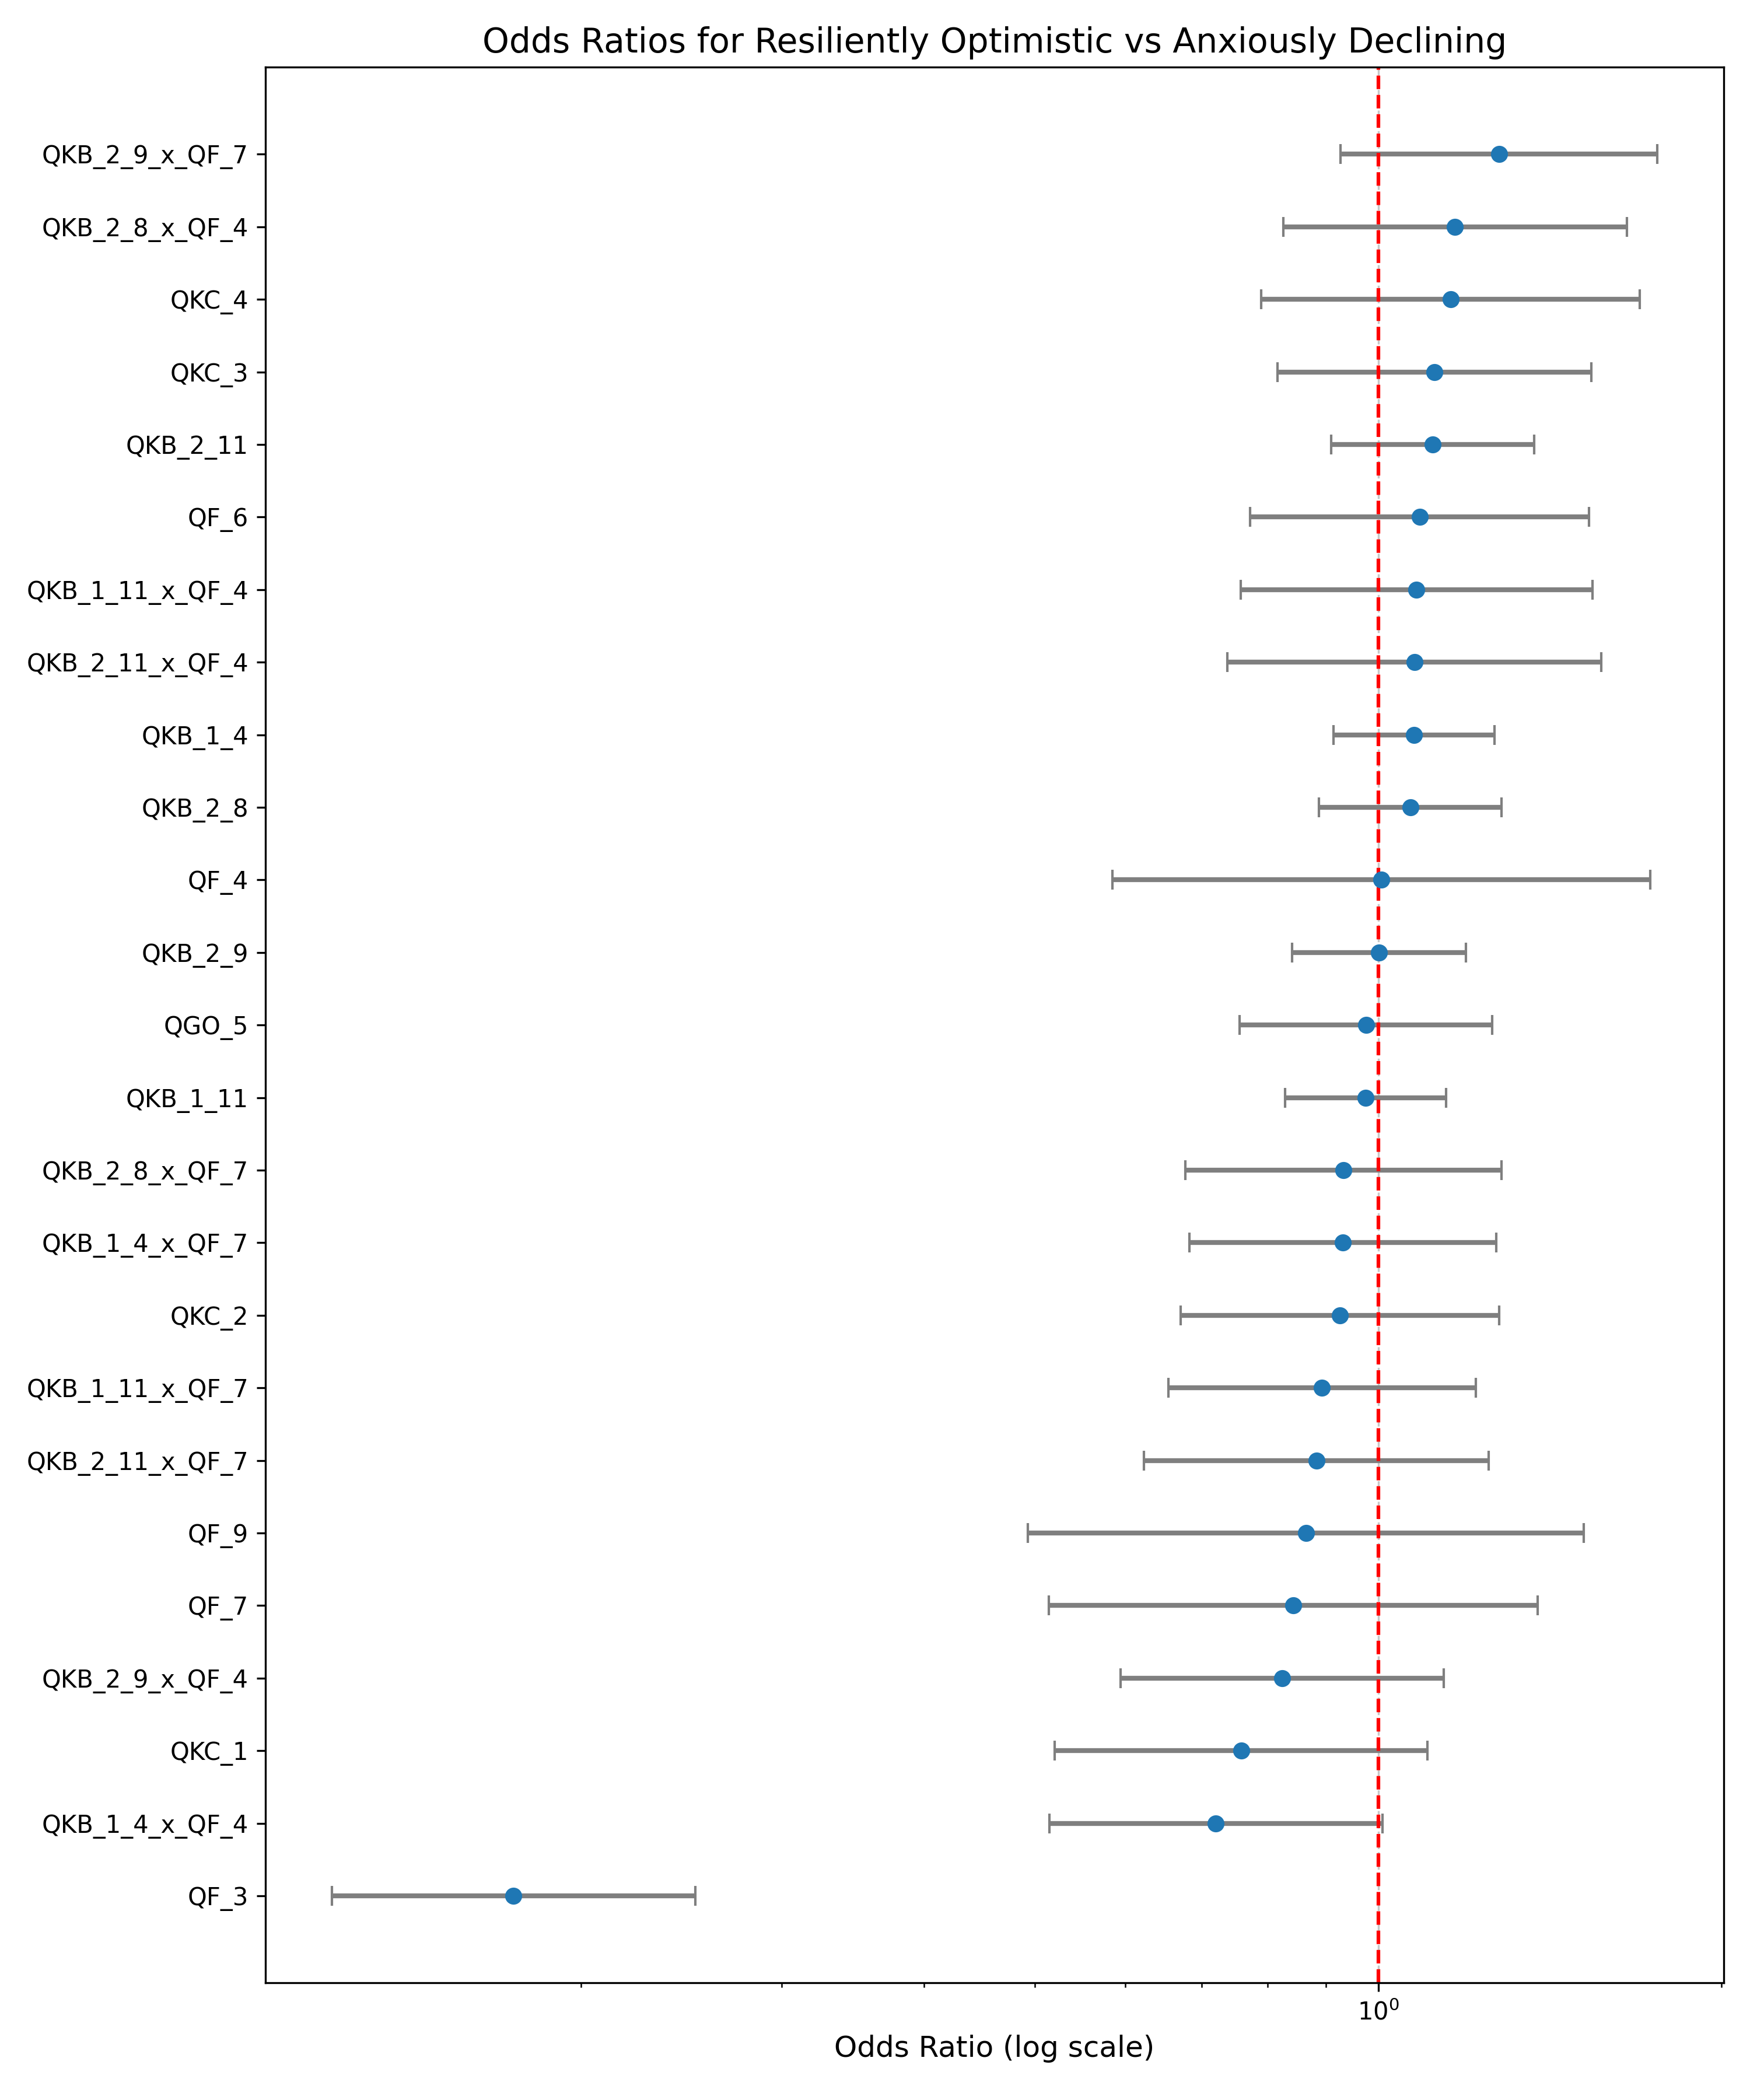
\includegraphics[width=0.6\textwidth]{../input_files/plots/step_5_forest_plot_odds_ratios_1776115179.png}
    \caption{Forest plot of odds ratios from the multinomial logistic regression, showing predictors of membership in the "Resiliently Optimistic" class relative to the "Anxiously Declining" class. Deterrents like worry about job loss (QF\_3) drastically decrease the odds of an optimistic outlook, while enablers like career progression incentives (QKC\_4) and employee involvement (QKB\_2\_11) increase them. Interaction effects show that autonomy over tools (QKB\_2\_9\_x\_QF\_7) can buffer the negative impact of privacy anxieties.}
    \label{fig:odds_ratios}
\end{figure}

\subsection{Simulating the impact of organizational policies}
To translate these regression findings into actionable insights, we conducted a Monte Carlo policy simulation to estimate the predicted probability of an average employee belonging to the "Resiliently Optimistic" class under different organizational scenarios. We specifically contrasted the effects of providing regular training with direct employee involvement in AI development.

The results, shown in Figure \ref{fig:policy_sim}, demonstrate that policies promoting active agency are far more effective than those focused on passive capability building. In the baseline scenario with neither training nor involvement, the predicted probability of being in the optimistic class is approximately 58\%. Introducing training alone provides only a marginal benefit. However, implementing a policy of direct employee involvement in AI development substantially increases this probability to over 65\%. This finding underscores that to foster psychological stability, organizations must grant employees an active, participatory role in the technological transition.

\begin{figure}[h!]
    \centering
    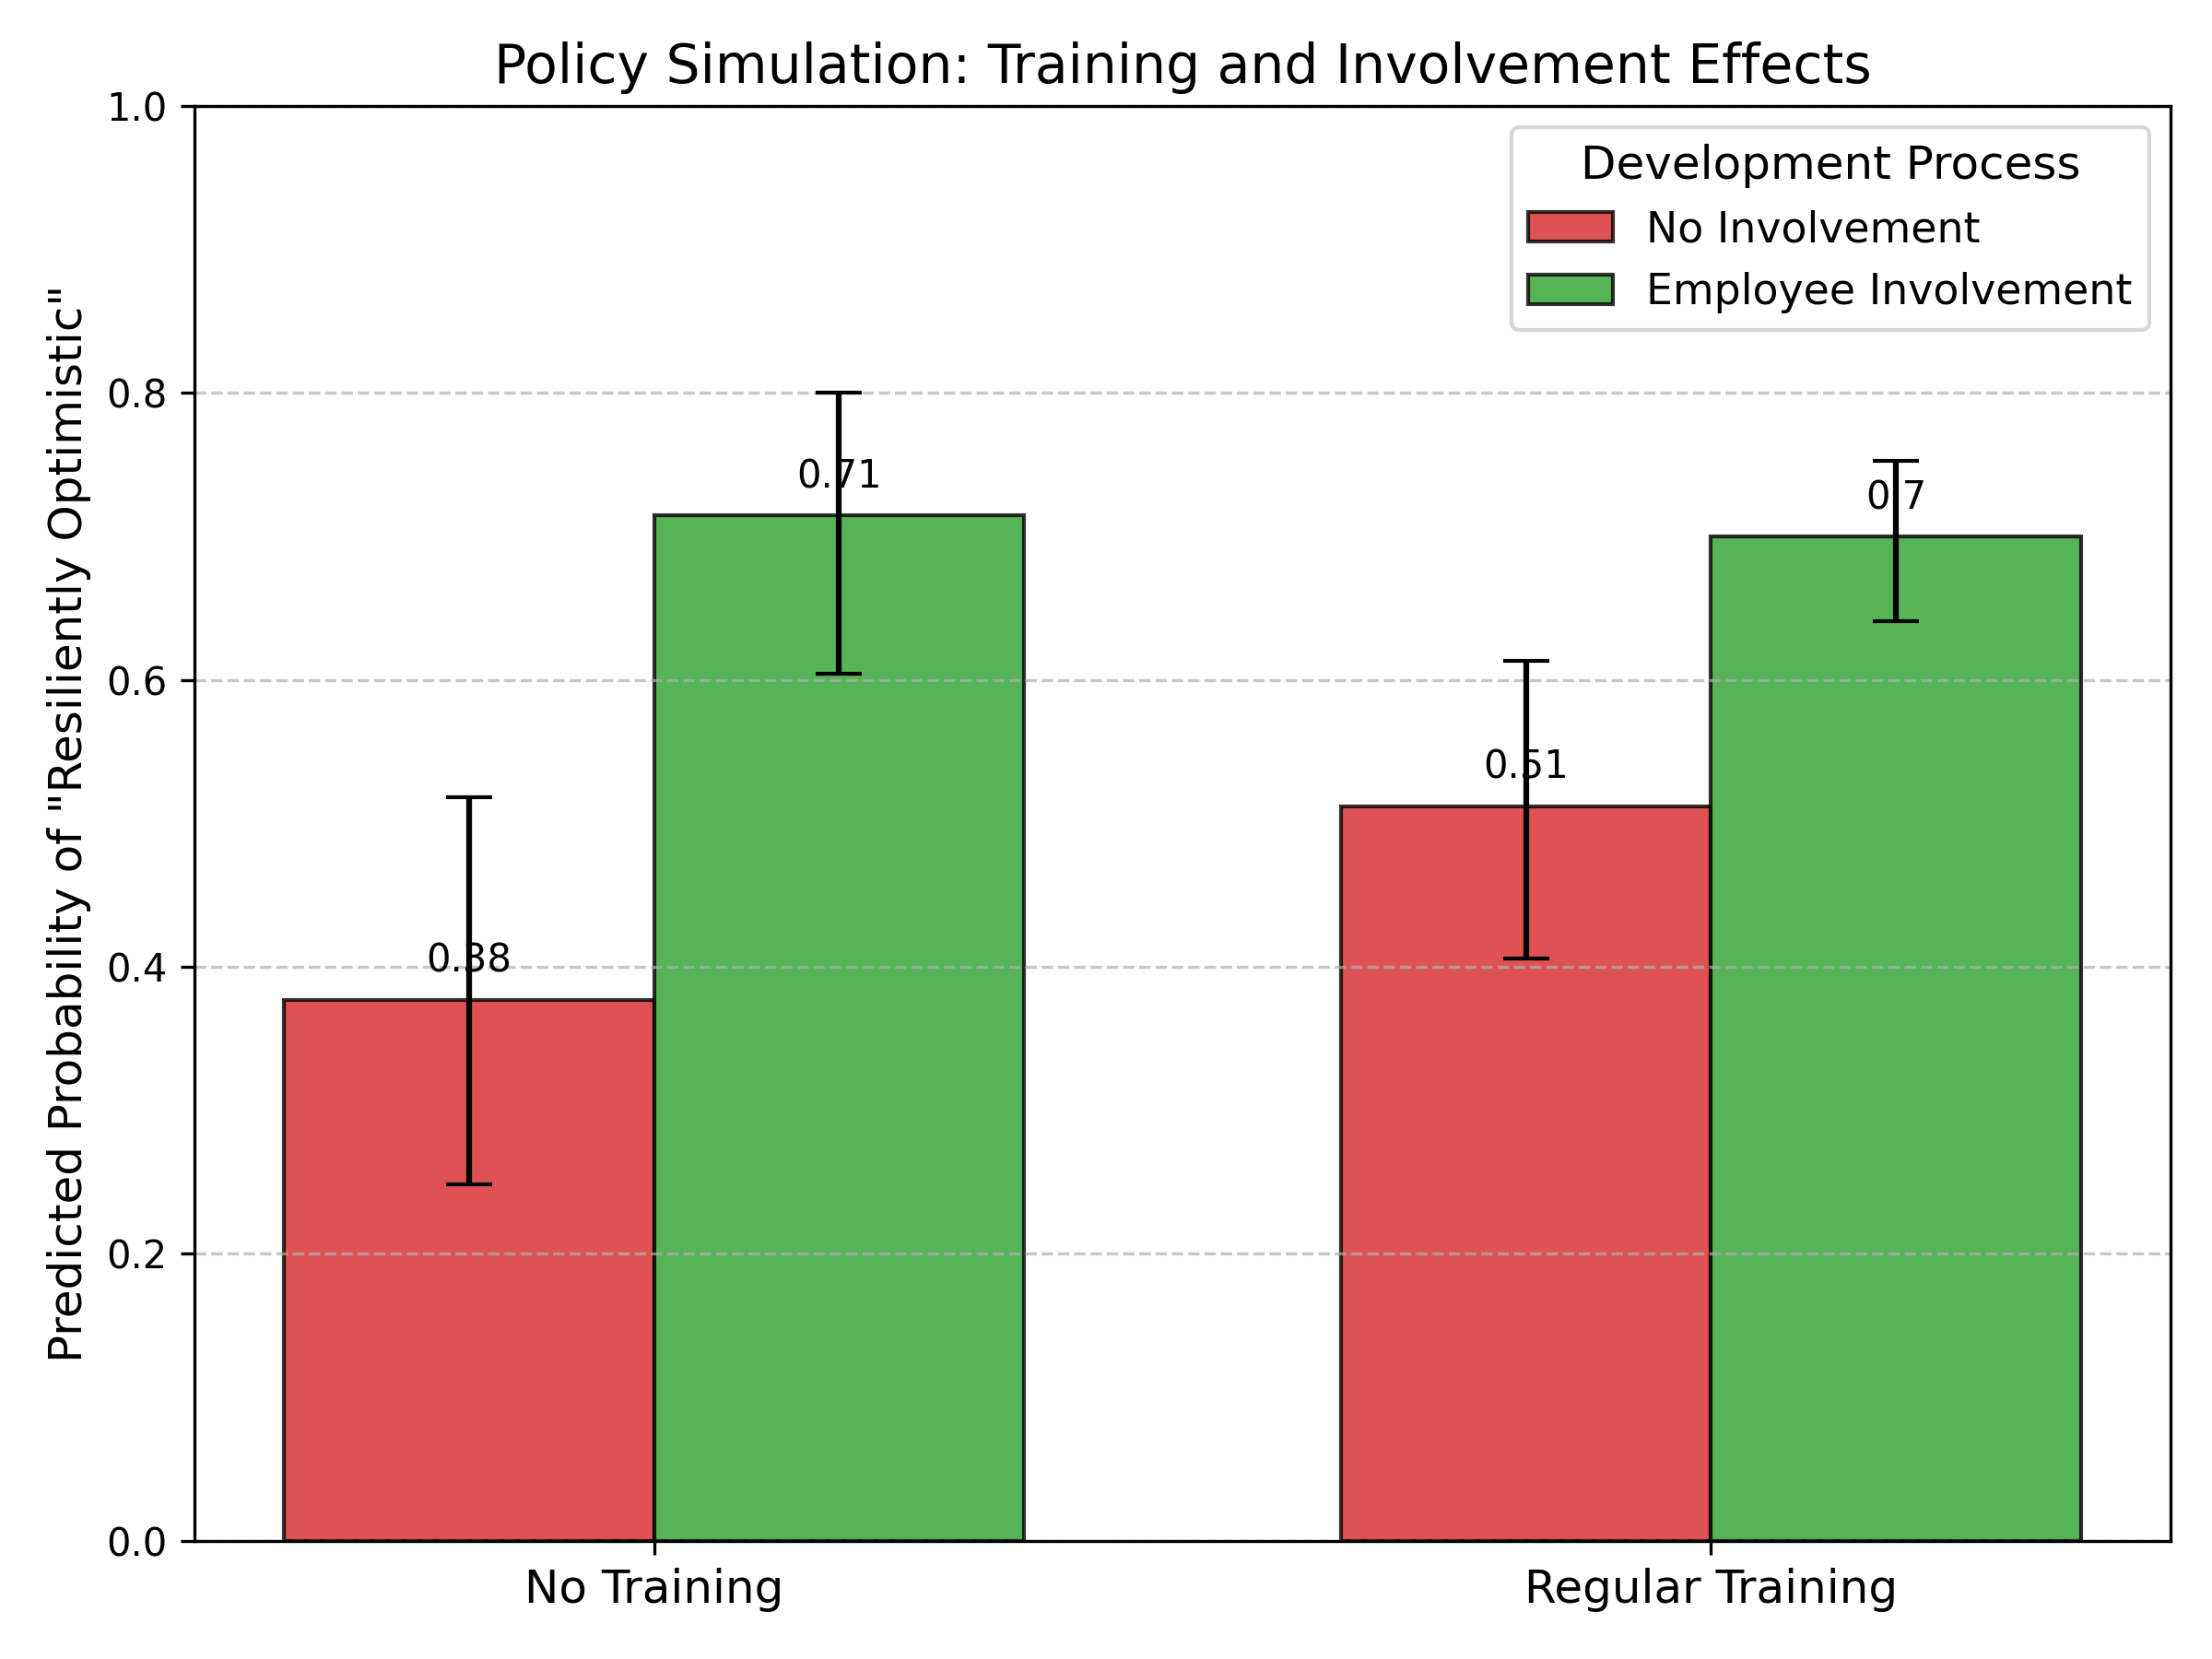
\includegraphics[width=0.6\textwidth]{../input_files/plots/step_6_policy_simulation_probabilities_1776115363.png}
    \caption{Predicted probability of membership in the "Resiliently Optimistic" class from a Monte Carlo policy simulation under four organizational scenarios. The simulation demonstrates that involving employees in the AI development process substantially elevates the probability of a positive outlook. In contrast, providing training alone yields only a marginal improvement, underscoring that active employee participation is a more potent catalyst for psychological stability than passive capability building.}
    \label{fig:policy_sim}
\end{figure}

\subsection{Robustness of findings}
To ensure the validity of our findings, we performed several robustness checks. First, a Variance Inflation Factor (VIF) analysis on the full design matrix of the multinomial model confirmed the absence of severe multicollinearity. All primary predictors exhibited VIF values well below the conventional threshold of 5.0 (e.g., employee involvement in development, VIF = 1.75; fear of accountability, VIF = 2.27).

Second, we conducted a tripartite sensitivity analysis to assess the stability of our results to the handling of "Not sure" responses in the dependent variables. The multinomial logistic regression was re-estimated on three sample variants: (1) the full sample (N=2603), (2) a sample excluding "Not sure" respondents (N=2538), and (3) the full sample with "Not sure" responses imputed to the modal value. The odds ratios for key predictors remained remarkably stable across all three specifications. For instance, the odds ratio for employee involvement (`QKB\_2\_11`) was highly consistent across the full (OR = 1.111), reduced (OR = 1.119), and imputed (OR = 1.120) samples. Similarly, the powerful negative effect of job loss worry (`QF\_3`) was stable (ORs of 0.174, 0.149, and 0.175, respectively). This stability confirms that our findings are robust and not systematically biased by respondent uncertainty.

\section{Conclusions}
\label{sec:conclusions}
This study sought to move beyond aggregate, variable-centered analyses of employee responses to Artificial Intelligence by adopting a person-centered approach to understand the heterogeneous nature of AI-induced job security perceptions. The central problem addressed is that monolithic views of the workforce obscure distinct psychological trajectories, leading to potentially misaligned organizational policies. To address this, we analyzed survey data from 2,603 employees in large global enterprises.

Our methodology first employed Latent Class Analysis to empirically identify unobserved subgroups based on employees' current and expected job security. This revealed a typology of three distinct classes: a majority ``Resiliently Optimistic'' cohort (60.9\%), a ``Stagnant Neutral'' group (26.5\%), and a significant ``Anxiously Declining'' minority (12.6\%). Subsequently, we used an Elastic Net regression for feature selection, followed by a multinomial logistic regression, to identify the organizational and psychological factors that predict membership in these classes.

The results demonstrate that an employee's trajectory is not predetermined but is strongly influenced by the organizational environment. Membership in the ``Resiliently Optimistic'' class was most strongly predicted by structural enablers that provide employees with agency and tangible value. These include direct involvement in the AI development process and non-monetary incentives such as peer recognition and learning certifications. Conversely, membership in the ``Anxiously Declining'' class was overwhelmingly driven by deterrents, with fear of job loss and privacy concerns being the most powerful predictors, capable of negating the positive effects of other organizational support mechanisms.

From these findings, we have learned several critical lessons. First, fostering psychological stability amidst technological change hinges less on abstract commitments to training and more on implementing participatory frameworks. Our policy simulation clearly showed that granting employees an active role in the AI transition is a far more potent catalyst for optimism than simply offering passive training programs. Second, the most effective organizational levers are those that decouple the evolution of job tasks from the perceived threat of job displacement by providing clear, tangible benefits and a sense of control. Ultimately, this research provides a data-driven framework for organizations, suggesting that the key to navigating the AI transition successfully is to proactively build an environment of agency, recognition, and empowerment, thereby steering the workforce toward resilience rather than anxiety.


\bibliography{bibliography}{}
\bibliographystyle{unsrt}

\end{document}
